\documentclass[12pt]{article}
\usepackage{graphicx,multicol}
\usepackage{url}
\title{An introduction to Blockchain technology}
\author{Mridul Gupta\\2019PCP5037 MNIT Jaipur}
\date{October, 2019}

\begin{document}

\maketitle
\section*{Abstract}
The aim of this paper is to provide an introduction and history of blockchain technology to people who consider venturing into the field of online transactions and security methods.

\begin{multicols}{2}

\section{Introduction}
Even though blockchain became popular in the recent years with the implementation as bitcoin\cite{Nak} and other cryptocurrency mechanisms coming up, the ideas has been around for years.

\section{Parts of Blockchain}
A blockchain is a type of distributed database, an atleast fifty years old idea, but the first mention of immutably chaning blocks of information using a cryptographic hash function appears in 1979 paper by Ralph Merkle\cite{Mer}.\par

Blockchain is a peer-to-peer distributed ledger that eliminates the need of a trusted third party in order to verify any piece of online data. The network itself acts as its own arbitrator to resolve any arbitration issues. As a result, blockchain makes complete non-reversible transactions possible\cite{Nak}.\par

Blockchain consists of cryptographically linked chain of blocks of data, each of which contains the cryptographic hash of the preceding block and the first block, usually called the genesis block, to create and immutable ledger.\par

Each node on the peer-to-peer network can append records to the ledger using transactions\cite{ieee}. Blockchain protocol consists of \textit{access policy} to determine who may read the blocks. Blockchain also defines \textit{control policy} to define who may participate in the evolution of blocks and \textit{consensus policy} to determine which state of the blockchain is valid to resolve issues and conflicts\cite{Alan}\cite{Nak}.
\end{multicols}

\begin{figure}
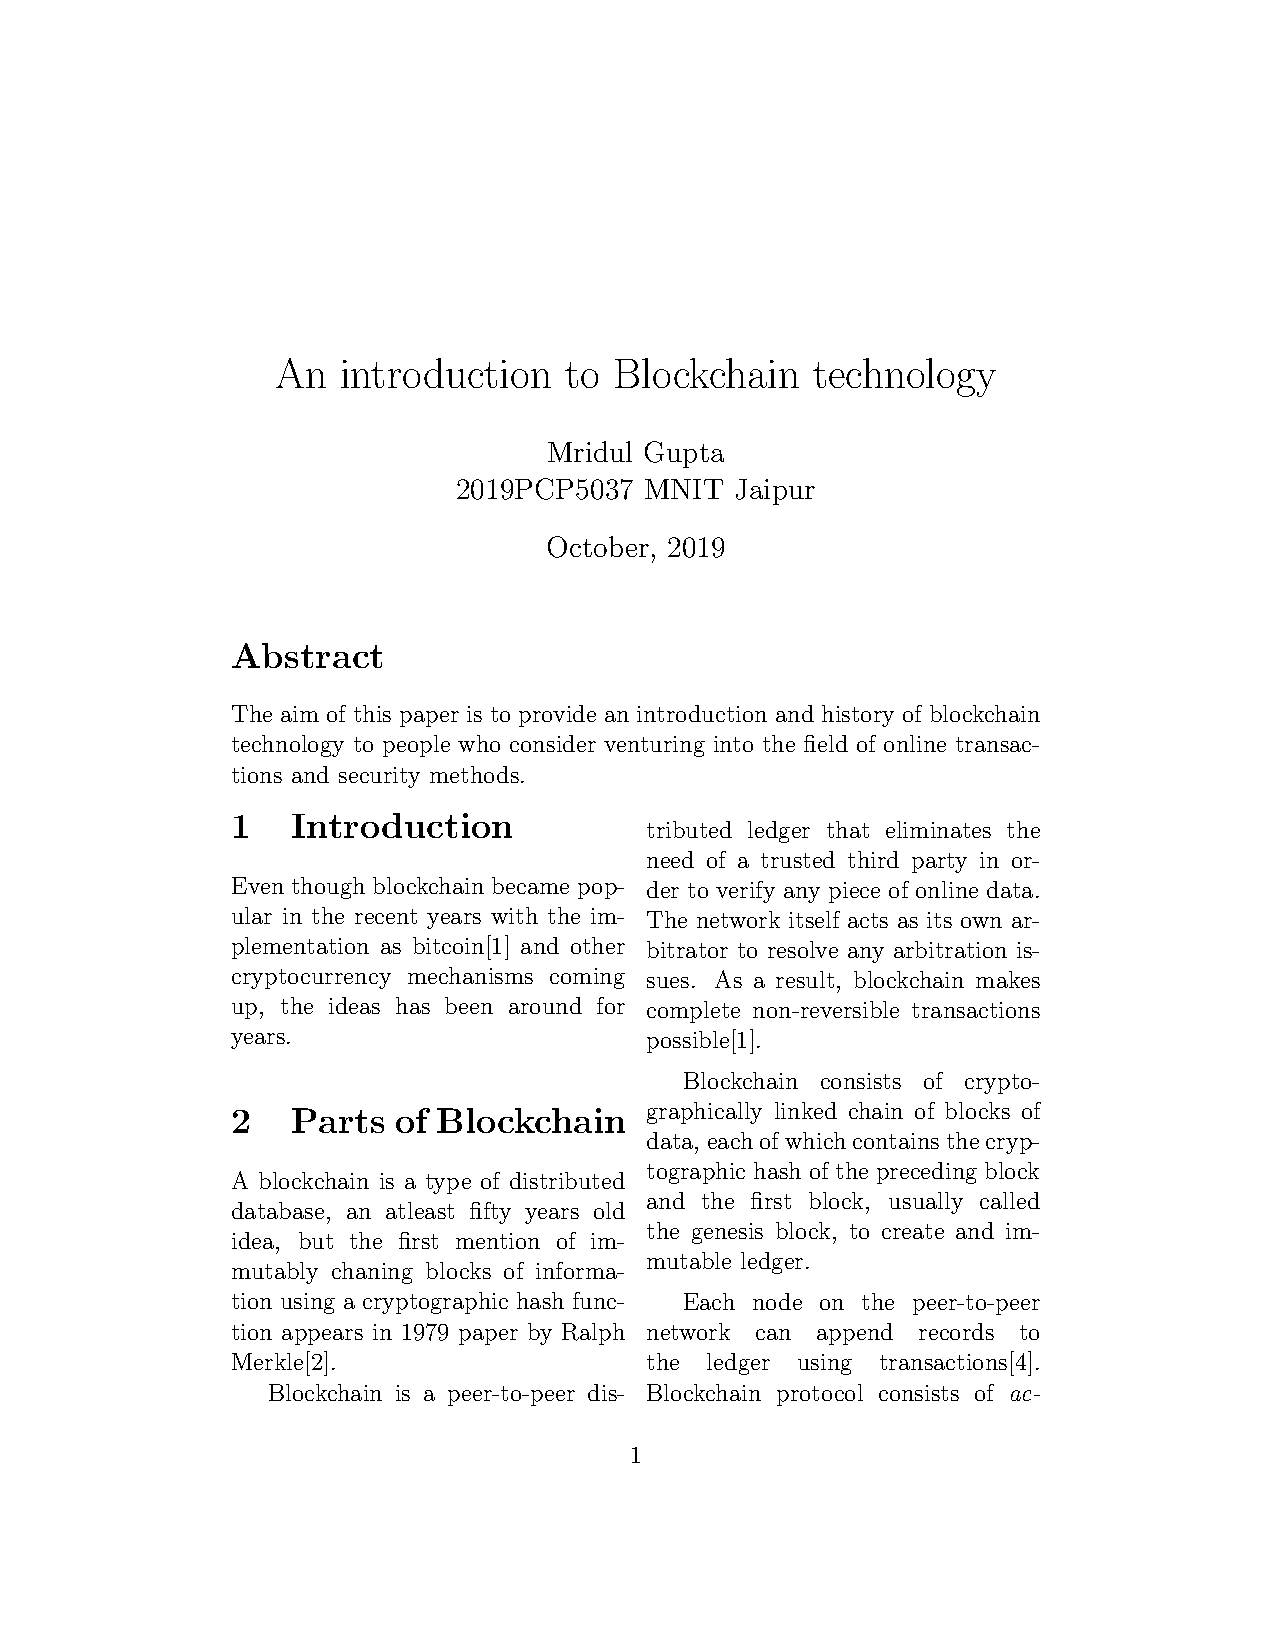
\includegraphics[width = \textwidth]{blockchain.png}
\caption{Blockchain components}
\end{figure}

\begin{table}
\begin{tabular}{|c || l|}
\hline
\hspace{5em}&\hspace{5em}\\
\textbf{1974} & Ralph Merkle, cryptographic puzzles \\
\textbf{1976} & Diffie Hellman, pioneering work on public-key cryptography\\
\textbf{1977} & Rivest, Shamir, Adleman, RSA cryptography created\\
\textbf{1979} & David Chaum, vaults and secret sharing (dissertation 1982)\\
\textbf{2002} & Adam Bach, Hashcash \\
\textbf{2008} & Satoshi Nakamoto, Bitcoin\\
\hline
\end{tabular}
\caption{timeline of selected blockchain discoveries}
\label{table:table-1}
\end{table}

\begin{multicols}{2}

\section{History of \\blockchain}
Any analysis of blockchain is incomplete without the understanding of the (at least) cryptographic concepts and papers listed in table \ref{table:table-1}, the discussion of which is beyond the scope here.\par

Blockchain borrows from various cryptographic ideas like public key cryptography, cryptographic hashing, digital signatures; and also from other computer science areas like database management systems, networking, peer-to-peer networks. Thus blockchain is a vast interdisciplinary that is difficult to understand.

\section{Future of blockchain}
Adaption of blockchains in e-Government, smart contracts, IoT, smart grids, smart cities, legal systems, public safety, public health, estate ownerships, property transactions, supply chain management, and many more is being considered rigorously. Many small start-ups are involved in studying applications of blockchain technology. The last decade has seen the growth of Bitcoin, and recently Bitcoin has gained enormous support from investors, thereby, raising its stock value. We believe the next decade will see the application of blockchain in other public and private sectors. This will have a significant enhancement in security and privacy of information.\cite{ieee}\par

There are three areas that require attention to make blockchain a viable technology to be used in broader applications. Firstly, the time complexity of various algorithms providing utility services within blockchain schemes must be significantly reduced to allow time-critical transactions to occur; secondly, the implementation of blockchain technology in distributed as well as in centralized computing environments must be possible; and, thirdly, the provision of security and privacy when blockchain technology is employed in open/public networks must be continuously re-addressed.\cite{ieee}\par

We believe practical and reliable solutions to the above challenges will expedite the use of blockchain technology and create a new capability within information networks of the future.\cite{ieee}
\end{multicols}
\begin{thebibliography}{9}

\bibitem{Nak}
Nakamoto Satoshi,
"Bitcoin: A peer-to-peer electronic cash system",
2008,
\url{https://bitcoin.org/bitcoin.pdf}

\bibitem{Mer}
Merkle R.C.,
"Secrecy, authentication, and public-key systems",
PhD Thesis,
Stanford University,
1979

\bibitem{Alan}
Sherman Alan, Farid Javani, Haibin Zhang, Enis Golaszewski,
"On the origin and variations of Blockchain Technologies",
2018

\bibitem{ieee}
"Blockchain: A Technical Overview - IEEE Internet Initiative",
\url{https://internetinitiative.ieee.org/newsletter/march-2018/blockchain-a-technical-review}
\end{thebibliography}
\end{document}